\documentclass[aspectratio=169]{beamer}

\usetheme{default}
\setbeamertemplate{navigation symbols}{}

\usepackage[T1]{fontenc}
\usepackage[utf8]{inputenc}
\usepackage{lmodern}
\usepackage{tikz}
\usepackage{xcolor}
\usepackage{hyperref}
\usetikzlibrary{arrows.meta,positioning,calc}
\tikzset{
  alt/.code args={<#1>#2#3}{\alt<#1>{\pgfkeysalso{#2}}{\pgfkeysalso{#3}}}
}

\definecolor{zkink}{HTML}{0F172A}
\definecolor{zkblue}{HTML}{12355B}
\definecolor{zkmuted}{HTML}{64748B}
\definecolor{zkrule}{HTML}{CBD5E1}
\definecolor{zkgreen}{HTML}{0E7C66}

\setbeamercolor{normal text}{fg=zkink,bg=white}
\setbeamercolor{frametitle}{fg=zkblue}
\setbeamercolor{structure}{fg=zkblue}
\setbeamertemplate{itemize item}{\raise0.18ex\hbox{\tikz\fill[zkblue] (0,0) circle (0.42ex);}}
\setbeamertemplate{enumerate item}{\color{zkblue}\insertenumlabel.}
\setbeamerfont{frametitle}{size=\Large,series=\bfseries}
\setbeamerfont{footline}{size=\tiny}
\setbeamersize{text margin left=0.62cm,text margin right=0.62cm}

\hypersetup{
  colorlinks=true,
  linkcolor=zkblue,
  urlcolor=zkblue
}

\newcommand{\sourcefoot}{}
\newcommand{\setsources}[1]{\renewcommand{\sourcefoot}{#1}}
\newcommand{\sourcetext}{\ifx\sourcefoot\empty\else Sources: \sourcefoot\fi}
\newcommand{\slidetitleline}{\vspace{0.06cm}{\color{zkrule}\rule{\linewidth}{0.5pt}}\vspace{-0.18cm}}
\newcommand{\labelhead}[1]{{\small\bfseries\color{zkblue}#1}\par\vspace{0.25em}}
\newcommand{\muted}[1]{{\color{zkmuted}#1}}
\newcommand{\takeaway}[1]{%
  \vspace{0.45em}%
  {\color{zkrule}\rule{\linewidth}{0.5pt}}\par
  \vspace{0.3em}%
  {\small\itshape\color{zkmuted}#1\par}}

\setbeamertemplate{frametitle}{
  \vspace{0.20cm}
  \insertframetitle\par
  \slidetitleline
}

\setbeamertemplate{footline}{
  \leavevmode
  \hbox{%
    \begin{beamercolorbox}[wd=.86\paperwidth,ht=3.4ex,dp=1.2ex,leftskip=.62cm]{footline}
      \color{zkmuted}\sourcetext
    \end{beamercolorbox}%
    \begin{beamercolorbox}[wd=.14\paperwidth,ht=3.4ex,dp=1.2ex,rightskip=.62cm plus1fil]{footline}
      \hfill\color{zkmuted}\insertframenumber\,/\,\inserttotalframenumber
    \end{beamercolorbox}%
  }
}

\title{Implementing ZK in swiyu}
\author{Antonio Kambir\'e}
\institute{zkSecurity}
\date{July 2026}

\begin{document}

% ---------------------------------------------------------------- 1. Title
\setsources{}
\begin{frame}[plain]
  \vspace{2.1cm}
  {\color{zkblue}\rule{0.15\paperwidth}{1.1pt}}\par
  \vspace{0.42cm}
  {\LARGE\bfseries\raggedright Implementing ZK in swiyu\par}
  \vspace{0.32cm}
  {\large\color{zkmuted}\raggedright
    Antonio Kambir\'e \quad \textbar \quad zkSecurity \quad \textbar \quad July 2026\par}
\end{frame}

% ------------------------------------------------- 2. How swiyu works
\setsources{\href{https://swiyu-admin-ch.github.io/introduction/}{swiyu Introduction}; \href{https://swiyu-admin-ch.github.io/technology-stack/}{Technology Stack}; \href{https://swiyu-admin-ch.github.io/open-source-components/}{Open Source Components}}
\begin{frame}{How swiyu works}
  \begin{minipage}{0.94\linewidth}
    \begin{itemize}
      \item Issuers are government agencies, companies, and institutions; holders
        use the swiyu wallet app; verifiers run swiyu Check (in person) or the
        Generic Verifier (online).
      \item The Base Registry publishes DIDs (\texttt{did:webvh}), public keys,
        and Token Status Lists; the Trust Registry says which real-world entity
        a DID belongs to.
      \item All beta components are open source; the wallet and verifier are the
        natural extension points.
    \end{itemize}
  \end{minipage}

  \vspace{0.85em}
  \centering
  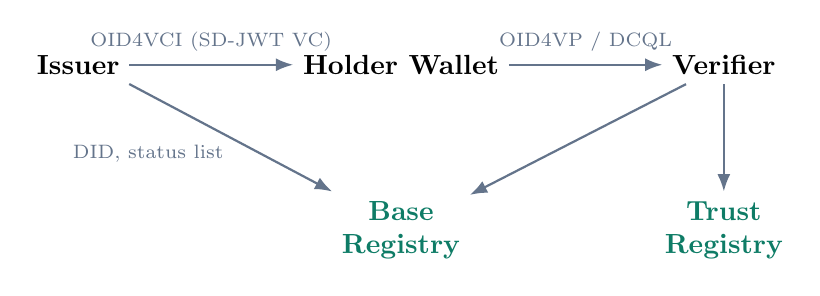
\begin{tikzpicture}[
    entity/.style={font=\bfseries, align=center},
    registry/.style={font=\bfseries, align=center, text=zkgreen},
    arrow/.style={-{Latex[length=2.2mm]}, thick, color=zkmuted},
    lab/.style={fill=white, inner sep=1.5pt, font=\scriptsize, text=zkmuted}
  ]
    \node[entity] (issuer) at (0,1.15) {Issuer};
    \node[entity] (wallet) at (4.1,1.15) {Holder Wallet};
    \node[entity] (verifier) at (8.2,1.15) {Verifier};
    \node[registry] (base) at (4.1,-0.95) {Base\\Registry};
    \node[registry] (trust) at (8.2,-0.95) {Trust\\Registry};

    \draw[arrow] (issuer.east) -- node[lab, above=3pt] {OID4VCI (SD-JWT VC)} (wallet.west);
    \draw[arrow] (wallet.east) -- node[lab, above=3pt] {OID4VP / DCQL} (verifier.west);
    \draw[arrow] (issuer.south east) -- node[lab, below left=1pt] {DID, status list} (base.north west);
    \draw[arrow] (verifier) -- (base);
    \draw[arrow] (verifier) -- (trust);
  \end{tikzpicture}
\end{frame}

% ------------------------------ 3. Infrastructure flow, over-18 example
\setsources{\href{https://swiyu-admin-ch.github.io/technology-stack/}{swiyu Technology Stack}; \href{https://www.rfc-editor.org/rfc/rfc9901.html}{RFC 9901}; \href{https://github.com/swiyu-admin-ch/swiyu-verifier\#digital-credentials-query-language-dcql}{swiyu Generic Verifier}}
\begin{frame}<1-4>{swiyu infrastructure flow: proving you are over 18}
  \begin{minipage}[t][2.9cm][t]{0.94\linewidth}
    \only<1>{%
      \labelhead{1. Issuance: inside the SD-JWT VC}
      \begin{itemize}
        \item The signed payload holds \texttt{iss}, \texttt{vct}, \texttt{exp},
          \texttt{status}, \texttt{cnf} (wallet key), and claim digests
          \texttt{\_sd: [H(d$_1$), H(d$_2$), ...]}.
        \item Each disclosure \texttt{[salt, "birthdate", "2001-05-03"]} stays
          with the wallet and hashes to a digest in \texttt{\_sd}.
        \item The signature is ES256 (ECDSA P-256) under the issuer's published
          DID key.
      \end{itemize}}
    \only<2>{%
      \labelhead{2. Request: OID4VP / DCQL}
      \begin{itemize}
        \item The verifier names a credential type and the claims it wants (here
          the \texttt{birthdate} of a Beta-ID) in a DCQL query.
        \item The request carries a fresh nonce and the verifier identity (audience).
        \item DCQL selects \emph{which claims to reveal}; it has no way to ask
          only ``over 18?''.
      \end{itemize}}
    \only<3>{%
      \labelhead{3. Presentation: selected disclosures + KB-JWT}
      \begin{itemize}
        \item The wallet returns the issuer-signed JWT and only the selected
          disclosures; the birthdate is revealed exactly.
        \item The KB-JWT is a signature with the \texttt{cnf} wallet key over the
          credential hash, nonce, and audience: it proves holder binding and
          prevents replay.
      \end{itemize}}
    \only<4>{%
      \labelhead{4. Verification: registries and status}
      \begin{itemize}
        \item Resolve the issuer DID in the Base Registry to get its public key;
          check the Trust Registry statement for who that DID is.
        \item Verify the ES256 signature, disclosure hashes, and KB-JWT.
        \item Fetch the Token Status List at the credential's status URI and
          check its index.
      \end{itemize}}
  \end{minipage}

  \vspace{0.35em}
  \centering
  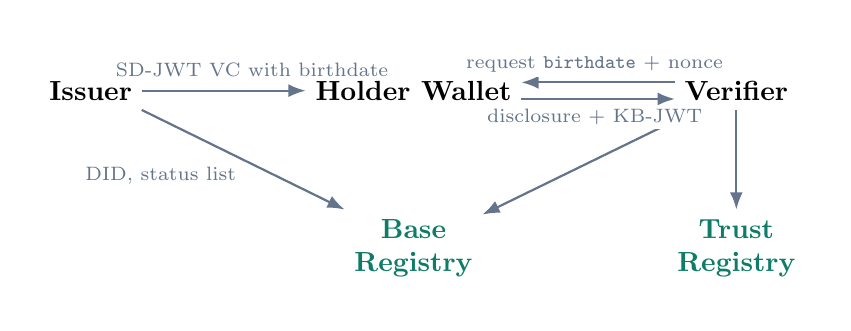
\begin{tikzpicture}[
    entity/.style={font=\bfseries, align=center},
    registry/.style={font=\bfseries, align=center, text=zkgreen},
    arrow/.style={-{Latex[length=2.2mm]}, thick, color=zkmuted},
    lab/.style={fill=white, inner sep=1.5pt, font=\scriptsize, text=zkmuted}
  ]
    \useasboundingbox (-0.8,-1.75) rectangle (9.3,1.75);
    \node[entity,alt=<1>{text=zkblue}{}] (issuer) at (0,0.95) {Issuer};
    \node[entity,alt=<3>{text=zkblue}{}] (wallet) at (4.1,0.95) {Holder Wallet};
    \node[entity,alt={<2,4>{text=zkblue}{}}] (verifier) at (8.2,0.95) {Verifier};
    \node[registry] (base) at (4.1,-1.05) {Base\\Registry};
    \node[registry] (trust) at (8.2,-1.05) {Trust\\Registry};

    \draw[arrow,alt=<1>{color=zkblue,very thick}{}] (issuer.east) -- (wallet.west);
    \draw[arrow,alt=<2>{color=zkblue,very thick}{}] ([yshift=3pt]verifier.west) -- ([yshift=3pt]wallet.east);
    \draw[arrow,alt=<3>{color=zkblue,very thick}{}] ([yshift=-3pt]wallet.east) -- ([yshift=-3pt]verifier.west);
    \draw[arrow,alt=<4>{color=zkblue,very thick}{}] (issuer.south east) --
      node[lab,below left=1pt] {DID, status list} (base.north west);
    \draw[arrow,alt=<4>{color=zkblue,very thick}{}] (verifier) -- (base);
    \draw[arrow,alt=<4>{color=zkblue,very thick}{}] (verifier) -- (trust);

    % edge labels drawn last so no arrow crosses them
    \node[lab,alt=<1>{text=zkblue}{}] at (2.05,1.22) {SD-JWT VC with birthdate};
    \node[lab,alt=<2>{text=zkblue}{}] at (6.4,1.28) {request \texttt{birthdate} + nonce};
    \node[lab,alt=<3>{text=zkblue}{}] at (6.4,0.62) {disclosure + KB-JWT};
  \end{tikzpicture}
\end{frame}

% ------------------------------------------------- 4a. Gap 1: no predicates
\setsources{\href{https://swiyu-admin-ch.github.io/threat-model/}{swiyu Threat Model}; \href{https://www.rfc-editor.org/rfc/rfc9901.html}{RFC 9901}}
\begin{frame}{Gap 1: no predicate proofs}
  \begin{columns}[T,onlytextwidth]
    \column{0.48\textwidth}
      \labelhead{What happens today}
      \begin{itemize}
        \item A bar only needs ``over 18'', but SD-JWT can either withhold the
          birthdate or reveal it exactly.
        \item So every age check hands the verifier a full, exact birthdate.
      \end{itemize}

    \column{0.48\textwidth}
      \labelhead{Why it matters}
      \begin{itemize}
        \item Verifiers can store what they receive indefinitely.
        \item Colluding verifiers can join their logs on revealed values; an
          exact birthdate is a strong join key. swiyu's threat model names
          verifier-verifier and issuer-verifier collusion explicitly.
      \end{itemize}
  \end{columns}

  \takeaway{Hiding a claim is not the same as proving something about it.}
\end{frame}

% ------------------------------------------- 4b. Gap 2: linkable material
\setsources{\href{https://swiyu-admin-ch.github.io/threat-model/}{swiyu Threat Model}; \href{https://www.eid.admin.ch/en/so-wird-die-e-id-unverknuepfbar-e}{e-ID batch issuance}; \href{https://raw.githubusercontent.com/swiyu-admin-ch/community/main/tech-concepts/e-id-key-management-batch-issuance-and-renewal.md}{Batch issuance whitepaper}}
\begin{frame}{Gap 2: presentations stay linkable}
  \begin{columns}[T,onlytextwidth]
    \column{0.48\textwidth}
      \labelhead{Stable identifiers in every presentation}
      \begin{itemize}
        \item Issuer signature bytes and salted claim digests repeat verbatim
          each time.
        \item The \texttt{cnf} holder public key is a stable identifier.
        \item A status-list URI + bit index unique to the credential lets
          verifiers re-check it later or cross-match it.
        \item Any of these seen twice links presentations, with nothing
          disclosed.
      \end{itemize}

    \column{0.48\textwidth}
      \labelhead{Current remediation: batch issuance}
      \begin{itemize}
        \item Issue many one-time credentials for the same attributes, each with
          a fresh holder key and status index; spend each once.
        \item Limits: reuse once the batch runs out, the issuer sees renewal
          timing, each status entry is still re-checkable, and Gap 1 remains.
      \end{itemize}
  \end{columns}

  \takeaway{Batch issuance reduces reuse linkage; it does not deliver full unlinkability.}
\end{frame}

% ---------------------------------------------------------------- 5. Why ZK
\setsources{\href{https://github.com/eu-digital-identity-wallet/eudi-doc-architecture-and-reference-framework/issues/200}{EUDI ARF issue \#200}; \href{https://github.com/eu-digital-identity-wallet/eudi-doc-standards-and-technical-specifications/blob/main/docs/technical-specifications/ts13-zksnarks.md}{EUDI TS13}; \href{https://swiyu-admin-ch.github.io/open-source-components/}{Open Source Components}}
\begin{frame}{Why ZK}
  \labelhead{Target primitive}
  swiyu SD-JWT VC $\rightarrow$ challenge-bound ZK proof that the credential was
  signed by a verifier-accepted issuer key/DID, is within its validity period,
  is held by a wallet controlling the \texttt{cnf} key, and satisfies a selected
  predicate: ``over 18'', not a birthdate.

  \vspace{0.25em}
  \begin{columns}[T,onlytextwidth]
    \column{0.48\textwidth}
      \labelhead{This closes both gaps}
      \begin{itemize}
        \item Gap 1: the verifier learns the predicate result, never the raw value.
        \item Gap 2: signature bytes, digests, and holder key stay inside the
          private witness; each proof is fresh.
      \end{itemize}

    \column{0.48\textwidth}
      \labelhead{And swiyu stays intact}
      \begin{itemize}
        \item New work sits in the open components: wallet-side proving and
          verifier-side validation.
        \item Issuance, registries, and trust semantics are untouched; ordinary
          presentations keep working alongside.
      \end{itemize}
  \end{columns}

  \takeaway{EUDI reached the same conclusion: ARF issue \#200 recommends
  anonymous credentials; TS13 explores circuit proofs over existing SD-JWT VCs.}
\end{frame}

% ------------------------------------------------------------- 6. OpenAC
\setsources{\href{https://github.com/privacy-ethereum/zkID}{zkID repo}; \href{https://eprint.iacr.org/2026/251}{OpenAC paper}; \href{https://github.com/microsoft/crescent-credentials}{Crescent}; \href{https://github.com/google/longfellow-zk}{Longfellow}; \href{https://github.com/succinctlabs/flock/blob/main/paper/flock-paper.pdf}{Flock paper}}
\begin{frame}{OpenAC (zkID) is the strongest starting point}
  \begin{columns}[T,onlytextwidth]
    \column{0.48\textwidth}
      \labelhead{Why it fits}
      \begin{itemize}
        \item \texttt{SD-JWT-P256} profile matches swiyu exactly: ES256 SD-JWT,
          disclosures, \texttt{cnf.jwk}.
        \item Prepare/Show: prove the credential once, then per-presentation
          challenge-bound predicate proofs.
        \item The other natural options, Crescent (generic JWT/mDL) and
          Longfellow (mdoc), fit less well.
        \item Mobile-practical: $\sim$3\,s one-time Prepare, $\sim$0.1\,s per
          Show (iPhone 17); Flock could cut hash costs further.
      \end{itemize}

    \column{0.48\textwidth}
      \labelhead{But not a direct drop-in}
      \begin{itemize}
        \item Align profile and claim normalization with \texttt{dc+sd-jwt} and
          the Beta-ID schema.
        \item Map issuer keys through swiyu DID resolution and trust statements.
        \item Define OID4VP/DCQL proof carriage; bind challenge and audience.
        \item ZK adds a new need: nullifiers for proof of unicity, so one
          credential cannot sign up twice.
        \item No public third-party audit yet.
      \end{itemize}
  \end{columns}
\end{frame}

% -------------------------------------------------------- 7. Prototype A
\setsources{\href{https://github.com/privacy-ethereum/zkID/blob/main/specs/1-openac/README.md}{OpenAC spec}; \href{https://swiyu-admin-ch.github.io/technology-stack/}{swiyu Technology Stack}}
\begin{frame}{Prototype A: SD-JWT-to-ZK overlay}
  \begin{columns}[T,onlytextwidth]
    \column{0.32\textwidth}
      \labelhead{Wallet Prepare}
      \begin{itemize}
        \item Parse the swiyu SD-JWT VC
        \item Verify ES256 signature and disclosures
        \item Normalize claims; cache the artifact
      \end{itemize}

    \column{0.32\textwidth}
      \labelhead{Wallet Show}
      \begin{itemize}
        \item Produce the challenge-bound device signature
        \item Prove the predicate
        \item Prove holder-key possession
      \end{itemize}

    \column{0.32\textwidth}
      \labelhead{Verifier}
      \begin{itemize}
        \item Validate proof and circuit/profile id
        \item Check issuer DID/key and trust policy
        \item Enforce challenge, audience, replay policy
      \end{itemize}
  \end{columns}

  \vspace{0.4em}
  \labelhead{Success}
  The verifier learns no raw birth date and no stable holder key for an age
  proof, receives no SD-JWT disclosure bundle, and cannot replay the proof;
  ordinary swiyu issuance remains unchanged.
\end{frame}

% -------------------------------------------------------- 8. Prototype B
\setsources{\href{https://github.com/privacy-ethereum/zkID/tree/main/revocation}{zkID revocation}; \href{https://github.com/eu-digital-identity-wallet/eudi-doc-standards-and-technical-specifications/blob/main/docs/technical-specifications/ts13-zksnarks.md}{EUDI TS13}}
\begin{frame}{Prototype B: status privacy extension}
  Compare three status designs for the Token Status List gap:

  \vspace{0.35em}
  \begin{itemize}
    \item \textbf{Sparse Merkle Tree}: publish a valid/revoked root; the wallet
      proves inclusion or non-membership locally. Measure proof size, update
      cost, witness generation.
    \item \textbf{zkID non-membership roots}: evaluate whether the wallet can
      avoid any credential-specific remote lookup during presentation.
    \item \textbf{EUDI TS13 adjacent-pair revocation}: hidden revocation handle
      bound into the credential; wallet proves its identifier lies between a
      signed revoked pair. Requires a status/issuance change.
  \end{itemize}

  \vspace{0.35em}
  \labelhead{Success}
  No stable status URI/index for the verifier, no presentation timing for the
  issuer or registry, practical mobile witness generation, and verifier checks
  simple enough for Generic Verifier integration.
\end{frame}

\end{document}
